\documentclass[12pt, titlepage]{article}

\usepackage{fullpage}
\usepackage[round]{natbib}
\usepackage{multirow}
\usepackage{booktabs}
\usepackage{tabularx}
\usepackage{graphicx}
\usepackage{float}
\usepackage{hyperref}

\hypersetup{
    colorlinks,
    citecolor=black,
    filecolor=black,
    linkcolor=red,
    urlcolor=blue
}

\usepackage[round]{natbib}
\usepackage{float}

%% Comments

\usepackage{color}

\newif\ifcomments\commentstrue %displays comments
%\newif\ifcomments\commentsfalse %so that comments do not display

\ifcomments
\newcommand{\authornote}[3]{\textcolor{#1}{[#3 ---#2]}}
\newcommand{\todo}[1]{\textcolor{red}{[TODO: #1]}}
\else
\newcommand{\authornote}[3]{}
\newcommand{\todo}[1]{}
\fi

\newcommand{\wss}[1]{\authornote{blue}{SS}{#1}} 
\newcommand{\plt}[1]{\authornote{magenta}{TPLT}{#1}} %For explanation of the template
\newcommand{\an}[1]{\authornote{cyan}{Author}{#1}}

%% Common Parts

\newcommand{\progname}{ProgName} % PUT YOUR PROGRAM NAME HERE
\newcommand{\authname}{Team \#, Team Name
\\ Student 1 name
\\ Student 2 name
\\ Student 3 name
\\ Student 4 name} % AUTHOR NAMES                  

\usepackage{hyperref}
    \hypersetup{colorlinks=true, linkcolor=blue, citecolor=blue, filecolor=blue,
                urlcolor=blue, unicode=false}
    \urlstyle{same}
                                


\begin{document}

\title{Verification and Validation Report: Artificial Neural Network (ANN)} 
\author{Tanya Djavaherpour}
\date{\today}
	
\maketitle

\pagenumbering{roman}

\section{Revision History}

\begin{tabularx}{\textwidth}{p{3cm}p{2cm}X}
\toprule {\bf Date} & {\bf Version} & {\bf Notes}\\
\midrule
Apr. 15, 2024 & 1.0 & Initial Draft\\
% Date 2 & 1.1 & Notes\\
\bottomrule
\end{tabularx}

~\newpage

\section{Symbols, Abbreviations and Acronyms}

\renewcommand{\arraystretch}{1.2}
\begin{tabular}{l l} 
  \toprule		
  \textbf{symbol} & \textbf{description}\\
  \midrule 
  T & Test\\
  \bottomrule
\end{tabular}\\

For more details, please refer to the SRS document \citep{SRS} 
\href{https://github.com/tanya-jp/ANN-CAS741/blob/main/docs/SRS/SRS.pdf}
{HERE}.

% \wss{symbols, abbreviations or acronyms -- you can reference the SRS tables if needed}

\newpage

\tableofcontents

\listoftables %if appropriate

\listoffigures %if appropriate

\newpage

\pagenumbering{arabic}

This document summarizes the Verification and Validation (VnV) 
processes applied to the ANN. It includes results from executing all 
test cases outlined in the VnV Plan \citep{VnVPlan}. Detailed outcomes for 
the functional and non-functional requirements are presented in Sections 
\ref{funcreq} and \ref{nfuncreq}, respectively. 
Additional sections provide comprehensive analyses of the test results.

\section{Functional Requirements Evaluation} \label{funcreq}
The functional requirements are evaluated in this section. 
A detailed description of all of these tests can be found in the VnV Plan 
\citep{VnVPlan}.

\subsection{T1}
This test checks the format of the input image to ensure it meets the size and 
format requirements and constraints. In this test, we verify that exceptions 
work properly, so that the end user will not be able to use files that are unacceptable.
The implemented test is available 
\href{https://github.com/tanya-jp/ANN-CAS741/blob/main/test/test_image_properties.py}{here}.
As it is indicated in the 
\href{https://github.com/tanya-jp/ANN-CAS741/blob/main/test/test_image_properties.log}{log file}, 
all of the tests are passed.

\subsection{T2}
This is a classifier test to make sure the implemented model can predict properly. 
For this purpose, a test is run using Pytest 
\citep{pytest}, 
which is available \href{https://github.com/tanya-jp/ANN-CAS741/blob/main/test/test_classifier.py}{here}. 
The result of this test is accessible 
\href{https://github.com/tanya-jp/ANN-CAS741/blob/main/test/test_classifier.log}{here}.
As it is indicated in the result file, all the tests are passed.

\section{Nonfunctional Requirements Evaluation} \label{nfuncreq}
The nonfunctional requirements are evaluated in this section.

\subsection{Accuracy}

The accuracy results are shown in \autoref{Accuracy} and the cost values
are indicater in Figure \ref{FigUH}. 
Also, accuracy results are accessible 
\href{https://github.com/tanya-jp/ANN-CAS741/blob/main/test/training_res.txt}{here}.

\begin{table}[h!]
  \begin{center}
  \begin{tabular}{ |c|c|}
  \hline
  Dataset & Accuracy \\
  \hline
  train data & 22.234 \%\\
  \hline
  test data & 21.959 \%\\
  \hline
  \end{tabular}
  \caption{Accuracy Results}
  \label{Accuracy}
  \end{center}
  \end{table}
		
  \begin{figure}[H]
    \centering
    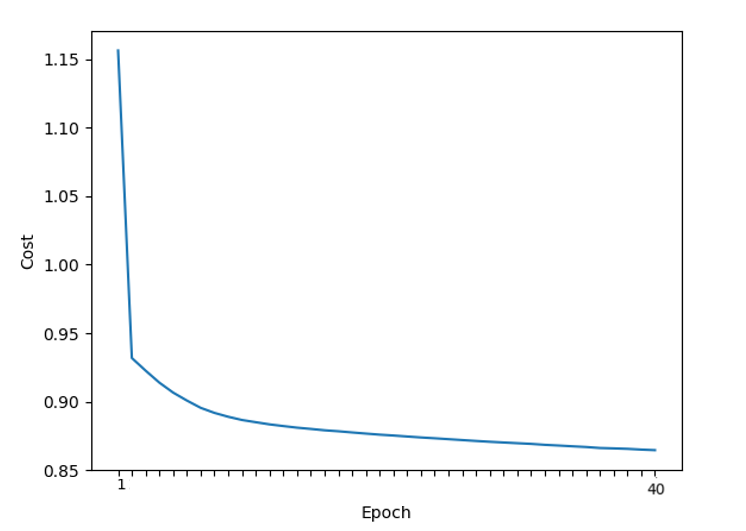
\includegraphics[width=0.5\textwidth]{Cost.png}
    \caption{Cost Value over 40 Epochs}
    \label{FigUH}
    \end{figure}

\subsection{Usability}

As the author has not yet received any feedback from usability surveys, 
reporting about this area is postponed to future drafts.

\subsection{Maintainability}

As it is mentioned in the VnV Plan \citep{VnVPlan}, 
Pylint \citep{pylint} library checked the quality of all of the modules.
Furthermore, we conducted Walkthrough Meetings to identify areas 
for improvement in system maintainability and documentation.

\subsection{Portability}

We tested this system on Windows and MacOS devices and it could pass
all the tests on bothh of them.

\subsection{User Interaction Efficiency}

This area will be discussed in future drafts since the author has 
not yet received feedback from end users.

	
\section{Comparison to Existing Implementation}	
This project is a re-implementation of a previous one, originally developed in a 
Jupyter Notebook without distinct modules. Also, in previous implementation the model was not
saved, whcih means there was not any feature for classifying uploaded images. 

The previous model was trained on only 4 classes, while we trained this model 
on ten different classes, including airplane, 
automobile, bird, cat, deer, dog, frog, horse, ship, and truck. 
The previous implementation has the accuracy of 45\%. In this project, 
after increasing the number of classes the reached accuracy is as shown in 
\autoref{Accuracy}.

In ANN, we expanded our dataset by 2.5 times and initially 
anticipated a proportional decrease in model accuracy, specifically expecting it to 
drop to almost 18\% (45 divided by 2.5) of its original value. However, the observed 
decline in accuracy was significantly less than predicted, indicating a 
robustness in our model that can handle increased data variability effectively. 
This unexpected outcome not only validates our approach but also highlights the 
enhanced generalization capability of our model, underscoring clear progress in 
our project objectives. 
 
\section{Unit Testing}
The following section includes different unit tests as described in the VnV Plan \citep{VnVPlan}. 
All the unit tests and their results are available 
\href{https://github.com/tanya-jp/ANN-CAS741/tree/main/test}{here}. 
As you can see, all of the tests are passed.

\subsection{ ANN Control Module Unit Test}
This unit test ensures that the main function of the software wokrs properly.
This function includes two parts: \textbf{Training Model} and 
\textbf{Classifying the Input Image}. This test is available 
\href{https://github.com/tanya-jp/ANN-CAS741/blob/main/test/control_unit.py}{here} and 
the results are shown \href{https://github.com/tanya-jp/ANN-CAS741/blob/main/test/control_unit.log}{here} 
with the OK received result.

\section{Changes Due to Testing}

During testing, there were no significant changes. 
The majority of the changes were related to exceptions. 
\href{https://github.com/tanya-jp/ANN-CAS741/commit/80cba12a28de6732807168bea3d07c342d0dbc4c}{This commit}
contains these changes.

\section{Automated Testing}

All the module are tested with Pylint \citep{pylint}.
Additionally, the unit tests and Pytest \citep{pytest} are 
applied on modules that are available on 
\href{https://github.com/tanya-jp/ANN-CAS741/tree/main/test}{GitHub repository}.
		
\section{Trace to Requirements}
The traceability between tests cases and requirements is displayed in \autoref{Traceability}.

\begin{table}[h!]
  \begin{center}
  \begin{tabular}{ |l|c|c|c|c|c|c|c|c|c|c}
  \hline
   & R1 & R2 & R3 & NFR1 & NFR2 & NFR3 & NFR4\\
  \hline
  T1 & X & X & & & & &\\
  \hline
  T2 & & & X & & & &\\
  \hline
  T3 & & & & X & &  & \\
  \hline
  T4 & & & & & X & & \\
  \hline
  T5 & & & & & & X &\\
  \hline
  T6 & & & & & & & X\\
  \hline
  \end{tabular}
  \caption{Tracebility between test cases and requirements}
  \label{Traceability}
  \end{center}
  \end{table}
		
\section{Trace to Modules}	
\autoref{tab:tc-traceability-module} indicates the traceability between tests and modules.
\begin{table}[h!]
  \begin{center}
  \begin{tabular}{ |l|c|c|c|c|c|c|c|c|c| }
  \hline
   & M2 & M3 & M4 & M5 & M6 & M7 & M8 & M9 & M10\\
  \hline
  T1 & & & & & X & & & &\\
  \hline
  T2 & & X & X & X & & & & & X\\
  \hline
  test-id1 - test-id2 & X & & & & & & & &\\
  \hline
  test-id3 - test-id10 & & X & & & & X & & & X\\
  \hline
  test-id11 - test-id18 & & & X & X & & X & & &\\
  \hline
  test-id19 - test-id26 & & & & & & & X & X &\\
  
  \hline
  \end{tabular}
  \caption{Tracebility between test cases and modules}
  \label{tab:tc-traceability-module}
  \end{center}
  \end{table}

\section{Code Coverage Metrics}

The result of code coverage is available 
\href{https://github.com/tanya-jp/ANN-CAS741/tree/main/test/htmlcov}{here}.
They have been tested based on unit tets and pytests.
The resuls are shown in \autoref{tab:code-coverage-metrics}. 
There are some important points about these results:

\begin{itemize}
  \item Having a main function to run the software is the reason control.py did not receive 100\%. 
  \item Because input\_prep.py uses input\_image methods, this module is not tested separately.
  \item Different methods of the train\_and\_test.py module are used in different 
  classes, and since the model can be run and tested, there is no special test.
\end{itemize}

\begin{table}[h!]
  \begin{center}
  \begin{tabular}{| c|c|c|c| c| }
  \hline
   \textbf{Name} &  \textbf{Stmts} &  \textbf{Miss} &  \textbf{Cover} & \textbf{Teset}\\ 
  \hline
  
  input\_image.py & 16 & 0 & 100\% & test\_image\_properties.py\\ 
  \hline
  classifier.py & 16 & 0 & 100\% & test\_classifier.py, output\_unit.py  \\ 
  \hline
  training\_model.py  & 15 & 0 & 100\% & test\_classifier.py, output\_unit.py, model\_unit.py  \\ 
  \hline
  data.py  & 57 & 0 & 100\% & data\_prep\_unit.py\\ 
  \hline
  control.py  & 18 & 1 & 94\% & control\_unit.py  \\ 
  \hline
  output.py & 38 & 0 & 100\% & output\_unit.py  \\ 
  \hline
  model.py  & 34 & 0 & 100\% & model\_unit.py\\ 
  % \hline
  % \textbf{Total} & 122 & 0 & 100\% \\ 
   
  \hline
  \end{tabular}
\caption{Tracebility Between Test Cases and Requirements}
\label{tab:code-coverage-metrics}
\end{center}
\end{table}
\bibliographystyle{plainnat}
\bibliography{../../refs/References}

% \newpage{}
% \section*{Appendix --- Reflection}

% The information in this section will be used to evaluate the team members on the
% graduate attribute of Reflection.  Please answer the following question:

% \begin{enumerate}
%   \item In what ways was the Verification and Validation (VnV) Plan different
%   from the activities that were actually conducted for VnV?  If there were
%   differences, what changes required the modification in the plan?  Why did
%   these changes occur?  Would you be able to anticipate these changes in future
%   projects?  If there weren't any differences, how was your team able to clearly
%   predict a feasible amount of effort and the right tasks needed to build the
%   evidence that demonstrates the required quality?  (It is expected that most
%   teams will have had to deviate from their original VnV Plan.)
% \end{enumerate}

\end{document}